
\section{Preliminaries: Pullbacks, Matching Families and Limits}\label{sec: tree co-decompositions}

\body{
    Throughout, all graphs are directed and allowed to contain loops, but not parallel edges. We describe a graph $G$ as a vertex set $V(G)$ along with an edge relation $E(G)\subseteq V(G)\times V(G)$. A \define{graph homomorphism} $\phi \colon G \to H$ is a function $\phi\colon V(G)\to V(H)$ so that if $(x,y)\in E(G)$, then $(\phi(x),\phi(y))\in E(H)$. We sometimes write the composition $g\circ f$ as $gf$. We think of undirected graphs $G$ as \textit{symmetric}, meaning that for each arc $(x,y) \in E(G)$ the arc $(y,x)$ is also in $G$. A \define{graph epimorphism} is a graph homomorphism which is surjective (as a function on vertex sets). See Hell and Ne{\v{s}}et{\v{r}}il~\cite{HellNesetril2004} for further background on homomorphisms. %We adopt the convention that \textit{all trees are directed} towards or away from a particular root.
}

\body{
    A \define{category} $\cat{C}$ is, roughly, a directed, reflexive graph equipped with a binary operation on edges called `composition'. Formally, it consists of a family of objects, morphisms $f:X\to Y$ between objects, an identity morphism $\cat{id}_X \colon X\to X$ for each object, and an associative composition law $g \circ f$  whenever the codomain of $f$ equals the domain of $g$, such that $f\circ \cat{id}_X=f$ and $\cat{id}_Y\circ f=f$. A \define{functor} $F \colon \cat{C} \to \cat{D}$ `is' a graph homomorphism: formally, it is a map sending objects (resp. arrows) in $\cat{C}$ to objects (resp. arrows) in $\cat{D}$ which preserves identities ($F(\cat{id}_X) = \cat{id}_{F(X)}$) and composition ($F(f \circ g) = F(f) \circ F(g)$). For background on category theory, appearing mostly in Section~\ref{sec: full FO}, we recommend Riehl~\cite{Riehl2016} and Awodey~\cite{Awodey2010}, and refer to Jacobs~\cite{JacobsCLTT} for the more advanced material on fibrations and categorical logic used later in the paper.
}

\body{
    Throughout the paper, when dealing with structures, we work with a fixed signature $\sigma$. Given a structure~$G$, we write $\pts{G}$ for the \define{underlying point set} of $G$. For example, if $\sigma$ is the signature of graphs encoded as a binary edge relation on a vertex set, then $\pts{G}$ is just $V(G)$; however, if $\sigma$ encodes graphs as an incidence relation between edges and vertices, then $\pts{G}$ is the set $E(G)\sqcup V(G)$. See Appendix~\ref{appendix:RS} for details.
}\label{para: prelim}

% TODO: Find an example showing that bounded tree co-width
% is not closed under taking subgraphs.
\vspace{-.5em}
\begin{minipage}[t]{0.70\textwidth}
\body{
Our constructions are based on \textit{pullbacks} (also known as \textit{fibered products}). Recall that, in any category~$\cat{C}$, given a \define{cospan}, that is a pair of morphisms with common codomain $X \xrightarrow{f} Z \xleftarrow{g} Y$, its \define{pullback} is an object $X\times_Z Y$ equipped with projection morphisms $X \xleftarrow{\pi_X} X\times_ZY \xrightarrow{\pi_Y} Y$ satisfying $f\pi_X=g\pi_Y$, and universal with this property: for any other object $W$ equipped with morphisms $u:W\to X$ and $v:W\to Y$ satisfying $fu=gv$, there exists a unique morphism $W\to X\times_ZY$ commuting with the projections.
}
\end{minipage}
\begin{minipage}[t]{0.20\textwidth}
% https://q.uiver.app/#q=WzAsNSxbMSwxLCJYXFx0aW1lc19aWSJdLFswLDEsIlgiXSxbMiwxLCJZIl0sWzEsMiwiWiJdLFsxLDAsIlciXSxbMCwxLCJcXHBpX1giLDJdLFswLDIsIlxccGlfWSJdLFsxLDMsImYiLDJdLFsyLDMsImciXSxbNCwxLCJ1IiwyXSxbNCwyLCJ2Il0sWzQsMCwiXFxleGlzdHMhIiwxXV0=
\[\hspace{1em}\begin{tikzcd}
	& W & \\
	X & {X\times_ZY} & Y \\
	& Z
	\arrow["u"', from=1-2, to=2-1]
	\arrow["{\exists!}"{description}, from=1-2, to=2-2]
	\arrow["v", from=1-2, to=2-3]
	\arrow["f"', from=2-1, to=3-2]
	\arrow["{\pi_X}"', from=2-2, to=2-1]
	\arrow["{\pi_Y}", from=2-2, to=2-3]
	\arrow["g", from=2-3, to=3-2]
\end{tikzcd}\]
\end{minipage}
\vspace{.4em}

\body{
In the category of sets, pullbacks have the concrete description $X\times_Z Y := \{(x,y)\in X\times Y : f(x)=g(y)\}$ with projections sending pairs to their first and second coordinates, respectively. The  {pullback} of $\sigma$-structures $G \xrightarrow{g} K \xleftarrow{h} H$ is the $\sigma$-structure $G\times_K H$ whose underlying set of points is $\pts{G\times_K H}:=\{(x,y)\in\pts{G}\times\pts{H}\mid g(x)=h(y)\},$ and whose relations are defined, for each $i\in I$, by $((x_1,y_1),\ldots,(x_{a_i},y_{a_i}))\in R_i^P
    \iff
    (x_1,\ldots,x_{a_i})\in R_i^G
    \ \text{and}\
    (y_1,\ldots,y_{a_i})\in R_i^H.$
Whether a given category $\cat{C}$ admits pullbacks is a property that must be checked. The category $\cat{Grph}$ of graphs and graph homomorphisms admits pullbacks, and we already unpacked this definition in Paragraph~\ref{para: pullback Leticia}; see Figure~\ref{fig:pullback} for an example.
}


\begin{figure}
    \begin{minipage}{0.58\textwidth}
        \includegraphics[width=\textwidth, page=8]{LLJ-figs.pdf}
    \end{minipage}%
    \hspace{\fill}
    \begin{minipage}{0.38\textwidth}
        \caption{Left: A cospan of graph epimorphisms, where the graph in the dashed box is the adhesion. Right: The cospan's pullback. Edge labels are in gray, vertex labels in black and no arrows on loops.}
    \label{fig:pullback}
    \end{minipage}%
\end{figure}

\begin{example}\label{ex:direct_product}
    The direct product $G\times H$ of a graph $G$ and a graph $H$ is equal to the pullback $G\times_o H$, where $o$ is the graph consisting of a single vertex with a loop.
\end{example}


\begin{comment}
\body{One can equivalently think of pullbacks of graphs (or relational structures), as follows. A vertex of $G\times_A H$ is a pair $(x,y)\in V(G)\times V(H)$ satisfying $g(x)=h(y)$, while an edge is a pair $(e,f)\in E(G)\times E(H)$ satisfying $g(e)=h(f)$ such that, if $e$ joins $x_1$ to $x_2$ in $G$ and $f$ joins $y_1$ to $y_2$ in $H$, then $(e,f)$ joins $(x_1,y_1)$ to $(x_2,y_2)$ in $G\times_A H$. We call the pair $(x,y)$ a \define{vertex matching family} of the pullback and the pair $(e,f)$ an \define{edge matching family}. This terminology is borrowed from sheaf theory (c.f.~Rosiak's textbook~\cite{Rosiak2022}) and can be easily lifed to co-decompositions as follows. 
}\label{para: matching families}

\begin{definition}\label{def: matching families}
Let $\Ta = (T, \{G_a\},\{g_t^e\})$ be a tree co-decomposition. A \define{matching family} for $\Ta$ is a tuple of vertices $(x_t)_{t\in V(T)}$ such that for all edges $e = (s,t)$ of $T$, the images of $x_s$ and $x_t$ agree in the adhesion $G_e$; explicitly, $g_s^e(x_s) = g_t^e(x_t).$ The \define{limit} of $\Ta$, denoted $\lim \Ta$, is the graph whose vertices are the set of matching families of $\Ta$ and where there is an edge from $(x_t)_{t\in V(T)}$ to $(y_t)_{t\in V(T)}$ whenever $(x_t,y_t)$ is an edge in $G_t$ for every $t\in V(T)$. We say that the co-decomposition $\Ta$ \define{decomposes} a graph $G$ if $G \cong \lim \Ta$.
\end{definition}
\end{comment}

\begin{definition}\label{def: matching families}
Let $\Ta = (T, \{G_a\},\{g_t^e\})$ be a tree co-decomposition. A \define{matching family} (cf.~\cite{Rosiak2022}) for $\Ta$ is a tuple of vertices $(x_t)_{t\in V(T)}$ such that for all edges $e = (s,t)$ of $T$, the images of $x_s$ and $x_t$ agree in the adhesion $G_e$; explicitly, $g_s^e(x_s) = g_t^e(x_t)$. The \define{limit} $\lim \Ta$ of $\Ta$ is the graph whose vertices are the set of matching families of $\Ta$ and where there is an edge from $(x_t)_{t\in V(T)}$ to $(y_t)_{t\in V(T)}$ whenever $(x_t,y_t)$ is an edge in $G_t$ for every $t\in V(T)$. We say that $\Ta$ \define{decomposes} a graph $G$ if $G \cong \lim \Ta$. The limit of a tree co-decomposition whose auxiliary tree is a single edge is exactly the pullback of the two bags over the adhesion.
\end{definition}

\begin{figure}
    \begin{minipage}{0.58\textwidth}
    \includegraphics[width=\textwidth, page=6]{LLJ-figs.pdf}
    \end{minipage}%
    \hspace{\fill}
    \begin{minipage}{0.38\textwidth}
    \caption{Two matching families: the red vertex and blue/double circled vertex. Since they differ in some bags, these are two different vertices in the limit. Since there is one in every bag, there is an edge from the red to blue vertex in the limit.}\label{fig:extension-picture}
    \end{minipage}%
\end{figure}

\body{
Given a co-decomposition $\Ta = (T, \{G_a\},\{g_t^e\})$ and a graph $G$ so that $G\cong\lim \Ta$, we can think of $\Ta$ as providing a coordinate system to the vertices of $G$, indexed by the nodes of $T$. Indeed, the graph $G$ can be viewed explicitly as a subgraph of the categorical product of all of the bags of $\Ta$.
}

\begin{observation}
    Let $\Ta=(T, \{G_a\},\{g_t^e\})$ be a tree co-decomposition. Then $\lim\Ta\subseteq\prod_{t\in V(T)}G_t$, where $\prod$ is the iterated direct product.
\end{observation}

\body{
The construction of \cref{def: matching families} satisfies the universal property characterizing the categorical limit (c.f.~Riehl~\cite{Riehl2016} for background), as we show below \footnote{Co-decompositions are categorical duals of \textit{structured decompositions}~\cite{BumpusKocsis2023} (or, in some sense equivalently, of cellular sheaves~\cite{Curry2014, HansenGhrist2019, Robinson2017}) and hence~\cite[Section 2.8]{BumpusKocsis2023} the dual of familiar tree decompositions. To make this explicit, denote coproducts as $A + B$ and let $T$ be a tree. The \define{barycentric subdivision} of $T$ is a finite category $\smallint T$ having $V(T) + E(T)$ as objects and having exactly one morphism from $e \in E(T)$ to $x \in V(T)$ whenever $e$ is incident with $x$. From this, it follows definitionally that \textit{there is a bijective correspondence between {tree co-decompositions} and diagrams of the form $d \colon (\smallint T)^{\op} \to \cat{Grph}$ with the property that, for any morphism $f \colon e \to x$ in $\smallint T$, the morphism $d(f)$ is epic.}
}.
}

\begin{definition}
A \define{cone} over a tree co-decomposition $\Ta=(T, \{G_a\},\{g_t^e\})$ consists of a graph $H$ together with a family of homomorphisms $\phi_a \colon H \to G_a$ for $a\in V(T)\cup E(T)$ such that for every node $t\in V(T)$ and $t$-incident edge $e$, we have that $\phi_e=g_t^e\circ\phi_t$. This, and matching families, yields the following imeditately. 
\end{definition}

\begin{proposition}\label{prop:universal}
Let $\Ta=(T, \{G_a\},\{g_t^e\})$ be a tree co-decomposition. Then $\lim \Ta$ is universal among cones over $\Ta$. That is, for every cone $(H,\{\phi_a\})$ there exists a unique graph homomorphism $u \colon H \to \lim \Ta$ commuting with the projection maps.
\end{proposition}
%\begin{proof} Given a cone $(H,\{\phi_a\})$, define $u(x)=(\phi_t(x))_{t\in V(T)}$ for every vertex $x\in V(H)$. The cone equations ensure that $u(x)$ is a matching family, and since every $\phi_t$ is a graph homomorphism, so is $u$. Uniqueness follows immediately from the projection maps. \end{proof}

\body{
Since the indexing graph is a tree, the limit of $\Ta$ can also be computed recursively by taking iterated pullbacks~\cite{Riehl2016}. This observation will be particularly useful in our algorithmic constructions. For completeness, we collect several structural results concerning co-decompositions in the appendices: we establish the relationship between tree co-width and tree-width (c.f.\ Appendix~\ref{appendix:tree-co-vs-tree}), we give a grammar characterization of path co-width (c.f.\ Appendix~\ref{appendix: grammar}) and we also show that every tree co-decomposition can be transformed into a \define{binary tree co-decomposition} without increasing its width (c.f. Appendix~\ref{appendix:binary}). Finally, in Appendix~\ref{appendix: tree shape important} we show that the restriction to tree-shaped diagrams is essential to obtaining a nontrivial width parameter: if arbitrary indexing shapes are allowed, every graph admits a co-decomposition of width at most three.
}






